\section{Self-Suspending Tasks in Multiprocessor Synchronization}
\label{sec:syn}

In this section, we consider the analysis of self-suspensions that arise on multiprocessors under P-FP scheduling when tasks synchronize access to shared resources (\eg, shared I/O devices, message buffers, or other shared data structures) with suspension-based locks (\eg, binary semaphores). As semaphores induce self-suspensions, some of the misconceptions surrounding the analysis of self-suspensions on uniprocessors unfortunately also spread to the analysis of  real-time locking protocols on partitioned multiprocessors.

In particular, the analysis framework to account for the additional interference due to \emph{remote blocking} first introduced by \cite{lakshmanan-2009}, and reused in several other works~\cite{zeng-2011,bbb-2013,yang-2013,kim-2014,han-2014,carminati-2014,yang-2014},  is unsafe, which we show with a counterexample in Section \ref{sec:counterexample}. Fortunately, as we will discuss in Section \ref{sec:safe_bound}, there are straightforward solutions based on the corrected response-time bounds discussed in Section \ref{sec:misconceptions}.

We begin with a review of existing analysis strategies for semaphore-induced suspensions on uniprocessors and partitioned multiprocessors. 
 

\subsection{Semaphores in Uniprocessor Systems}
\label{sec:sem-uni}

Under suspension-based locking protocol, tasks that are denied access to a shared resource are suspended. Interestingly, on uniprocessors, the resulting suspensions are \emph{not} considered to be \emph{self}-suspensions and can be accounted for more efficiently than general self-suspensions.

For example, consider semaphore-induced suspensions as they arise under the classic \emph{priority ceiling protocol} (PCP)~\cite{SRL:90}. Audsley et al.~\cite{audsley-1993} established that (in the absence of release jitter and assuming constrained deadlines) the response time of task $\tau_k$ under the PCP is given by the least non-negative $R_k \leq D_k$ that satisfies the following equation:
\begin{equation}
R_k = C_k+ B_k+\sum_{\tau_i \in hp(k)}\ceiling{\frac{R_k}{T_i}} C_i,
\label{eq:classic-pcp-rta}
\end{equation}
where $B_k$ denotes the maximum duration of \emph{priority inversion}~\cite{SRL:90} due to semaphore contention (\ie, the maximum amount of time that a pending job of $\tau_k$ is not scheduled while a lower-priority job executes). Notably, Dutertre~\cite{Du:99} later confirmed the correctness of this claim  with a formal, machine-checked proof using the PVS proof assistant. 

Comparing Eq. \eqref{eq:dynamic-correct} (general self-suspensions) with Eq.  \eqref{eq:classic-pcp-rta} (suspensions due to semaphores), it is apparent that Eq. \eqref{eq:classic-pcp-rta} is considerably less pessimistic since the ceiling term does not include $R_i$ or $D_i$. Intuitively, this difference is due to the fact that tasks incur blocking due to semaphores only if a local lower-priority task holds the resource (\ie, when the local processor is busy). In contrast, general self-suspensions may overlap with idle intervals.


\subsection{Semaphores in Partitioned Multiprocessor Systems}
\label{sec:sem-multi}

When suspension-based protocols, such as the \emph{multiprocessor priority ceiling protocol (MPCP)}~\cite{rajkumar-1990}, are applied under partitioned scheduling, resources are classified according to how they are shared: if a resource is shared by two or more tasks assigned to different processors, then it is called a \emph{global resource}, otherwise it is called a \emph{local resource}.

Similarly, a job is said to incur \emph{remote blocking} if it is waiting to acquire a global resource that is held by a job on another processor, whereas it is said to incur \emph{local blocking} if it is prevented from being scheduled by a lower-priority task on its local processor that is holding a resource (either global or local).

Regardless of whether a task incurs local or remote blocking, a waiting task always suspends until the contested resource becomes available. The resulting task suspension, however, is analyzed differently depending on whether a local or a remote task is currently holding the lock.

From the perspective of the local schedule on each processor, remote blocking is caused by external events (\ie, resource contention due to tasks on the other processors) and pushes the execution of higher-priority tasks to a later time point regardless of the schedule on the local processor (\ie, even if the local processor is idle). Remote blocking thus may cause additional interference on lower-priority tasks and must be analyzed as a self-suspension.

In contrast, local blocking takes place only if a local lower-priority task holds the resource (\ie, if the local processor is busy), just as it is the case with uniprocessor synchronization protocols like the PCP~\cite{SRL:90}. Consequently, local blocking is accounted for similarly to blocking under the PCP in the uniprocessor case (\ie, as in Eq. \eqref{eq:classic-pcp-rta}), and not as a general self-suspension (Eq. \eqref{eq:dynamic-correct}). Since local blocking can be handled similarly to the uniprocessor case, we focus on remote blocking in the remainder of this section.


A safe, but pessimistic strategy is to simply model remote blocking as computation, which is called \emph{suspension-oblivious analysis}~\cite{BA:10b}. By overestimating the processor demand of self-suspending, higher-priority tasks, the additional delay due to deferred execution is \emph{implicitly} accounted for as part of regular interference analysis. Block et al.~\cite{block-2007} first used this strategy in the context of partitioned and global \emph{earliest deadline first (EDF)} scheduling; Lakshmanan et al.~\cite{lakshmanan-2009} also adopted this approach in their analysis of ``virtual spinning,'' where tasks suspend when blocked on a lock, but at most one task per processor may compete for a global lock at any time. However, while suspension-oblivious analysis is conceptually straightforward, it is also subject to structural pessimism, and it has been shown that, in pathological cases, suspension-oblivious analysis can overestimate response times by a factor linear in both the number of tasks and the ratio of the largest and the shortest periods~\cite{wieder-2013}.

A less pessimistic alternative to suspension-oblivious analysis is to \emph{explicitly} bound the effects of deferred execution due to remote blocking, which is called \emph{suspension-aware analysis}~\cite{BA:10b}. Inspired by Ming's (flawed) analysis of self-suspensions  \cite{MingLiRTCSA1994}, Lakshmanan et al.~\cite{lakshmanan-2009} proposed such a response-time analysis framework that explicitly accounts for remote blocking.  Lakshmanan et al.'s  bound~\cite{lakshmanan-2009} was subsequently reused by several authors in
\begin{itemize}
\item \cite{zeng-2011} (Equation 9), \cite{han-2014} (Equation 5), and \cite{yang-2014} (Section 2.5) in the context of the MPCP, and
\item \cite{yang-2013} (Equation 6), \cite{bbb-2013} (Equation 1), \cite{carminati-2014} (Equations 3, 12, and 16), and \cite{kim-2014} (Equation 6)  in the context of other suspension-based locking protocols.
\end{itemize}

To state  Lakshmanan et al.'s claimed bound, some additional notation is required. In the following, let $B_k^r$ denote an upper bound on the maximum remote blocking that a job of $\tau_k$ incurs, let $C_k^{\ast} = C_k + B_k^r$, and let $\fun{lp(k)}$ denote the tasks with lower priority than $\tau_k$, respectively. Furthermore, let $P(\tau_k)$ denote the tasks that are assigned on the same processor as $\tau_k$, let $s_k$ denote the maximum number of critical sections of $\tau_k$, and let $C_{l,j}^{\prime}$ denote an upper bound on the execution time of the $j$\xth critical section of $\tau_l$.

Assuming constrained deadlines, Lakshmanan et al.~\cite{lakshmanan-2009} claimed that the response time of task $\tau_k$ is bounded by the least non-negative $R_k \leq D_k$ that satisfies the equation
\begin{equation}
\label{eqn:wcrt}
R_k = C_k^{\ast} + \sum_{\tau_i \in \fun{hp(k)} \cap P(\tau_k)} \left \lceil \frac{R_k + B_i^r}{T_i} \right \rceil \cdot C_i + s_k \sum_{\tau_l \in \fun{lp(k)} \cap P(\tau_k)} \max_{1 \leq j < s_l} C_{l,j}^{\prime}.
\end{equation}



In Eq. \eqref{eqn:wcrt}, the additional interference on $\tau_k$ due to the lock-induced deferred execution of higher-priority tasks is supposed to be captured by the term ``$+ B^r_i$'' in the interference bound  $\left \lceil \frac{R_k + B_i^r}{T_i} \right \rceil \cdot C_i$,  similarly to the misconception discussed in Section~\ref{sec:wrong-jitter-dynamic}. For completeness, we show with a counterexample that Eq. \eqref{eqn:wcrt} yields an unsafe bound in certain corner cases.

\subsection{A Counterexample}
\label{sec:counterexample}

We show the existence of a schedule in which a task that is considered schedulable according to Eq. \eqref{eqn:wcrt} misses a deadline.

%\begin{figure}[!ht]
\begin{center}
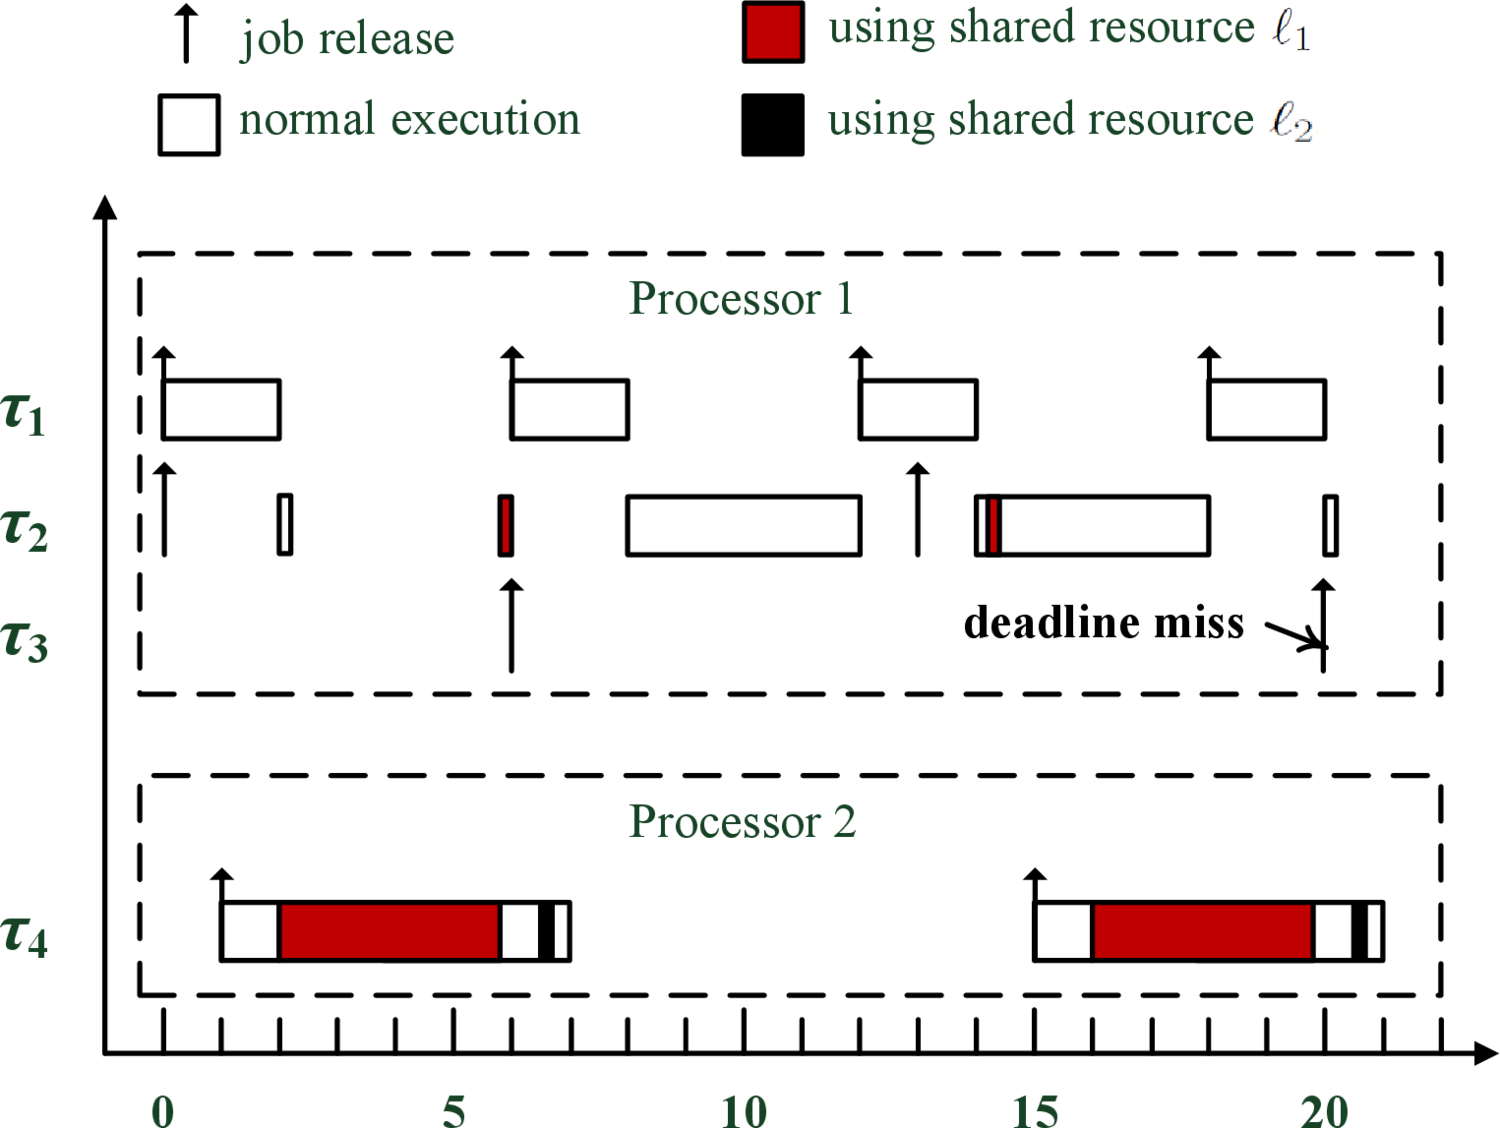
\includegraphics[width=12cm]{Counterexample}
\caption{An example schedule in which $\tau_3$ misses a deadline. 
}
\label{fig:counterexample_protocol}
\end{center}
\end{figure}


\begin{table}[t]
\centering
    \begin{tabular}{|c|c|c|c|c|c|} 
 \hline
        $\tau_k$ & $C_k$ & $T_k$ ($= D_k$) & $s_k$ & $C_{k,1}^{\prime}$ & Processor\\
        \hline
        $\tau_1$ & 2             & 6  & 0 & $-$ & $1$\\ 
        $\tau_2$ & $4+6\epsilon$ & 13 & 1 & $5\epsilon$& $1$\\
        $\tau_3$ & $\epsilon$    & 14 & 0 & $-$ & $1$\\
        $\tau_4$ & 7             & 14 & 1 & $4-4\epsilon$ & $2$\\ 
        \hline
    \end{tabular}
    \caption{Task parameters for the counterexample in Section~\ref{sec:counterexample}.}
    \label{table:parameters}
\end{table}

Consider four implicit deadline sporadic tasks ${\tau_1, \tau_2, \tau_3, \tau_4}$ with parameters as listed in Table \ref{table:parameters}, indexed in decreasing order of priority, that are scheduled on two processors using P-FP scheduling. Tasks $\tau_1$, $\tau_2$ and $\tau_3$ are assigned to processor 1, while task $\tau_4$ is assigned to processor 2.

Each job of $\tau_2$ has one critical section (($s_2 = 1$) of length at most $5\varepsilon$ (\ie, $C_{2,1}^{\prime} = 5\varepsilon$), where $0 < \varepsilon \leq 1/3$, in which it accesses a global shared resource $\res_1$.

Each job of $\tau_4$ has one critical section ($s_4 = 1$) of length at most $4-4\varepsilon$ (\ie, $C_{4,1}^{\prime} = 4-4\varepsilon$), in which it also accesses $\res_1$.

Consider the response time of $\tau_3$. Since $\tau_3$ does not access any global resource and because it is the lowest-priority task on processor $1$, it does not incur any global or local blocking (\ie, $B_3^r = 0$ and $s_3 \sum_{\tau_l \in \fun{lp}(3) \cap P(\tau_3)} \max_{1 \leq j < s_l} C_{l,j}^{\prime} = 0$). With regard to the remote blocking incurred by each higher-priority task, we have $B_1^r = 0$ because $\tau_1$ does not request any global resource. Further, each time when a job of $T_2$ requests $\res_1$, it may be delayed by $\tau_4$ for a duration of at most $4-4\varepsilon$. Thus the maximum remote blocking of $\tau_2$ is bounded by $B_2^r = C_{4,1}^{\prime} = 4-4\varepsilon$.\footnote{In general, the upper bound on blocking of course depends on the specific locking protocol in use, but in this example, by construction, the stated bound holds under any reasonable locking protocol. Recent surveys of multiprocessor semaphore protocols may be found in \cite{bbb-2013,yang-2015}.} Therefore, according to Eq. \eqref{eqn:wcrt}, the response time of $\tau_3$ is claimed by  Lakshmanan et al.'s analysis~\cite{lakshmanan-2009} to be bounded by
\begin{equation*}
R_3 = \varepsilon + \left \lceil \frac{8+7\varepsilon + 0}{6} \right \rceil \cdot 2 + \left \lceil \frac{8+7\varepsilon + 4-4\varepsilon}{13} \right \rceil \cdot (4+6\varepsilon) = 8+7\varepsilon.
\end{equation*}

\begin{figure}[t]
\centering
\def\uxfpga{0.4cm}
\scalebox{0.9}{
\begin{tikzpicture}[x=\uxfpga,y=\uy,auto, thick]
	\draw[->] (-0.4,0) -- coordinate (xaxis) (24,0) node[anchor=north]{$t$};
    \foreach \x in {0,2,...,22}{
         \draw[-,below](\x,0) -- (\x,-0.3) node[] {\pgfmathtruncatemacro\yi{\x} \yi};
    }
    	\foreach \x in {0,1,...,21}{
         \draw[-,very thin,lightgray, dashed](\x,0.3) -- (\x,9.75);
	}	
	\foreach \x in {-0.4,22}{
		\draw[-,thin,gray] (\x,0) -- (\x,2.25);
		\draw[-,thin,gray] (\x,2.7) -- (\x,9.75);
	}
	\foreach \y in {2.25,2.7,9.75}{
		\draw[-,thin,gray] (-0.4,\y) -- (22,\y);
	}
	\foreach \y in {3,5,7}{
		\draw[] (0,\y) -- (22,\y);
	}	
    \node[anchor=east] at (13, 1.5) {Processor 1};
    \node[anchor=east] at (13, 9.25) {Processor 2};

	\begin{scope}[shift={(0,0)}]
	    \node[anchor=east] at (-0.5, 0.5) {$\tau_4$};
		\foreach \x in {1,15}{
			\draw[->] (\x,0) -- (\x,1.75);
        		\node[task7, minimum width=\uxfpga, anchor=south west] at (\x, 0){\footnotesize};         
        		\node[task9, minimum width=3.4*\uxfpga, anchor=south west] at (\x+1, 0){\footnotesize};
        		\draw[] (\x+4.4,1.03)--(\x+6,1.03);
        		\draw[] (\x+6,0)--(\x+6,1.03);
		}
	\end{scope}
        
    \begin{scope}[shift={(0,3)}]
		\node[anchor=east] at (-0.5, 0.5) {$\tau_3$};    
    		\draw[->] (6,0) -- (6,1.75);
    		\draw[<-,red] (20,0) -- (20,1.2);
    		\node[anchor=east,red] at (21, 1.5) {miss};
    	\end{scope}
        
    \begin{scope}[shift={(0,5)}]    
        \node[anchor=east] at (-0.5, 0.5) {$\tau_2$};
        \draw[->] (0,0) -- (0,1.75);
        \draw[->] (13,0) -- (13,1.75);
        \foreach \y in {0.3,0.5,0.7}{
        		\draw[] (2.15,\y) -- (5.5,\y);
        	}
        \draw[] (2,1.03)--(2.15,1.03);
        \draw[] (2.15,0)--(2.15,1.03);
        \draw[] (2,0) -- (2,1.03);
        \node[task9, minimum width=0.1*\uxfpga, anchor=south east] at (6.05, 0){\footnotesize};
        \node[task7, minimum width=4*\uxfpga, anchor=south west] at (8, 0){\footnotesize}; 
        \draw[] (14,1.03)--(14.15,1.03);
        \draw[] (14,0)--(14,1.03);
        \node[task9, minimum width=0.1*\uxfpga, anchor=south west] at (14.15, 0){\footnotesize};
        \draw[] (14.7,1.03)--(18,1.03);
        \draw[] (18,0)--(18,1.03);
        \node[task7, minimum width=0.1*\uxfpga, anchor=south west] at (20, 0){\footnotesize};
	\end{scope}
	
	\begin{scope}[shift={(0,7)}]
        \node[anchor=east] at (-0.5, 0.5) {$\tau_1$}; 
        \foreach \x in {0,6,...,18}{
        		\draw[->] (\x,0) -- (\x,1.75);
		    \node[task7, minimum width=2*\uxfpga, anchor=south west] at (\x, 0){\footnotesize};
		}
	\end{scope}
\end{tikzpicture}}       
\caption{A schedule where $\tau_3$ misses a deadline.}
\label{fig:counterexample_protocol}
\end{figure}

\ifpaper
%\begin{figure}[t]
%  \centering
%  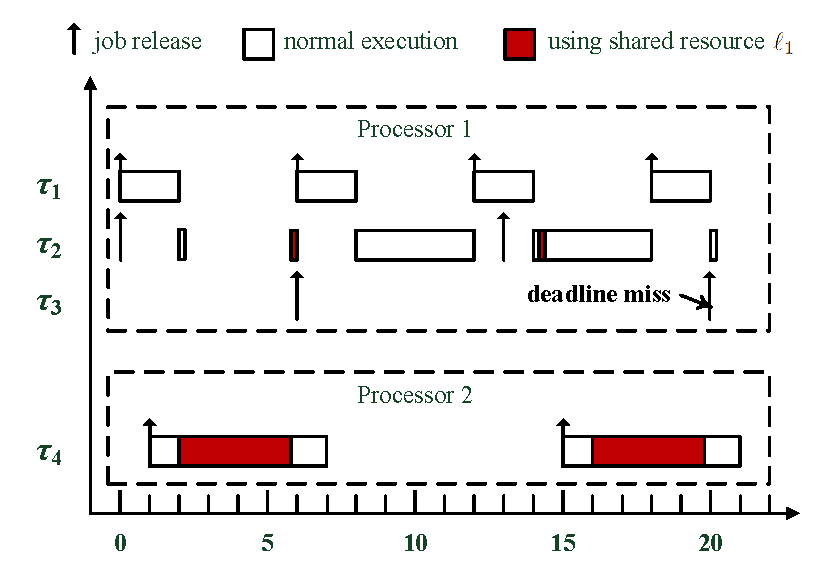
\includegraphics[width=0.85\linewidth]{../figures/Counterexample1/Counterexample1.pdf}
%  \caption{An example schedule where $\tau_3$ misses a deadline.}\label{fig:counterexample_protocol}
%\end{figure}
 \fi

However, there exists a schedule, shown in Fig. \ref{fig:counterexample_protocol}, in which a job of task $\tau_3$ arrives at time $6$ and misses its absolute deadline at time $20$. This implies that Eq. \eqref{eqn:wcrt} does not always yield a sound response-time bound. 

The misconception here is to account for remote blocking (\ie, $B_i^r$), which is a form of self-suspension, as if it were release jitter. However, it is not sufficient to account for self-suspensions as release jitter, as already explained in Section~\ref{sec:wrong-jitter-dynamic}.

\subsection{Incorrect Contention Bound in Interface-Based Analysis}

A related problem affects an \emph{interface-based analysis}  proposed by Nemati et al.~\cite{NBN:11}. Targeting \emph{open} real-time systems with globally shared resources (\ie, systems where the final task set composition is not known at analysis time, but tasks may share global resources nonetheless), the goal of the interface-based analysis is to extract a concise abstraction of the constraints that need to be satisfied  to guarantee the schedulability of all tasks. In particular, the analysis seeks to determine the \emph{maximum tolerable blocking time}, denoted $\fun{mtbt}_k$, that a task $\tau_k$ can tolerate without missing its deadline. 

Recall from classic uniprocessor time-demand analysis \cite{lehoczky-1989} that, \emph{in the absence of jitter or self-suspensions}, a task $\tau_k$ is considered schedulable if
\begin{equation}
\label{eqn:rbf-1}
\exists t \in (0,D_k]: \fun{rbf_{FP}}(k,t) \leq t, 
\end{equation}
where $\fun{rbf_{FP}}(k,t)$ is the \emph{request bound function} of $\tau_k$, which is given by

\begin{equation}
\label{eqn:rbf-2}
\fun{rbf_{FP}}(k,t) = C_k + B_k + \sum_{\tau_i \in \fun{hp}(k)} \left \lceil \frac{t}{T_i} \right \rceil \cdot C_i.
\end{equation}

Starting from Eq. \eqref{eqn:rbf-1}, Nemati et al.~\cite{NBN:11} first  replaced $\fun{rbf_{FP}}(k,t)$ with its definition, and then substituted  $B_k$ with $\fun{mtbt}_k$. Solving for $\fun{mtbt}_k$ yields:
\begin{equation}
\label{eqn:bloc-tolerate}
\fun{mtbt}_k = \max_{0<t \leq D_k} \left\{ t - \left( C_k + \sum_{\tau_i \in \fun{hp}(k)} \left \lceil \frac{t}{T_i} \right \rceil \cdot C_i \right) \right\}.
\end{equation}

However, based on the example in Section \ref{sec:counterexample}, we can immediately infer that Eqs. \eqref{eqn:rbf-1} and \eqref{eqn:rbf-2}, which ignore the effects of deferred execution due to remote blocking, are unsound in the presence of global locks. Consider $\tau_3$ in the previous example (with parameters listed in Table \ref{table:parameters}). According to Eq.~\eqref{eqn:bloc-tolerate}, we have $\fun{mtbt}_3 \geq 12 - (\epsilon + \lceil 12 / 6 \rceil \cdot 2 + \lceil 12 / 13 \rceil \cdot (4+6\epsilon)) = 4-7\epsilon$ (for $t=12$), which implies that $\tau_3$ can tolerate a maximum blocking time of at least $4-7\epsilon$ without missing its deadline. However, this is not true since $\tau_3$ can miss its deadline even without incurring any blocking, as shown in Fig. \ref{fig:counterexample_protocol}. 

\subsection{A Safe Response-Time Bound}
\label{sec:safe_bound}

In Eq. \eqref{eqn:wcrt}, the effects of deferred execution  are accounted for similarly to release jitter. However, it is not sufficient to count the duration of remote blocking as release jitter, as already explained in Section~\ref{sec:wrong-jitter-dynamic}.

A straightforward fix is to replace $B_i^r$ in the ceiling term (\ie, the second term in Eq. \eqref{eqn:wcrt}) with a larger, safe value such as $D_i$  or $R_i - C_i$ if $R_i \leq T_i$ (as discussed in Section~\ref{sec:wrong-jitter-dynamic}): assuming constrained deadlines, the response time of task $\tau_k$ is bounded by the least non-negative $R_k \leq D_k$ that satisfies the equation
\begin{equation}
\label{eqn:wcrt-pfp-fixed}
R_k = C_k^{\ast} + \sum_{\tau_i \in \fun{hp(k)} \cap P(\tau_k)} \left \lceil \frac{R_k + R_i - C_i}{T_i} \right \rceil \cdot C_i + s_k \sum_{\tau_l \in \fun{lp(k)} \cap P(\tau_k)} \max_{1 \leq j < s_l} C_{l,j}^{\prime}.
\end{equation}


Similarly, the term $\sum_{\tau_i \in \fun{hp}(k)} \lceil t / T_i \rceil \cdot C_i$ in Eqs. \eqref{eqn:rbf-2} and \eqref{eqn:bloc-tolerate} should be replaced with $\sum_{\tau_i \in \fun{hp}(k)} \lceil (t+D_i) / T_i \rceil \cdot C_i$ or $\sum_{\tau_i \in \fun{hp}(k)} \lceil (t+R_i-C_i) / T_i \rceil \cdot C_i$ to properly account for the deferred execution of higher-priority tasks.

Finally, the already mentioned papers~\cite{zeng-2011,bbb-2013,yang-2013,kim-2014,han-2014,carminati-2014,yang-2014} that reused Eq. \eqref{eqn:wcrt} can be fixed by simply using Eq. \eqref{eqn:wcrt-pfp-fixed} instead, because they merely reused the unsafe suspension-aware response-time bound introduced in \cite{lakshmanan-2009} without further modifications (\ie, the actual contributions in \cite{zeng-2011,bbb-2013,yang-2013,kim-2014,han-2014,carminati-2014,yang-2014} remain unaffected by this correction).
  
  


%%% Local Variables:
%%% mode: latex
%%% TeX-master: "JRTS/JRTS.tex"
%%% End:


  